\chapter{Register Transfer Level}
\section{Core}
This is the higher level of the design. It's interface with the external world and the data and the instruction memory, which are not reported in this document.
\begin{figure}[H]
\centering
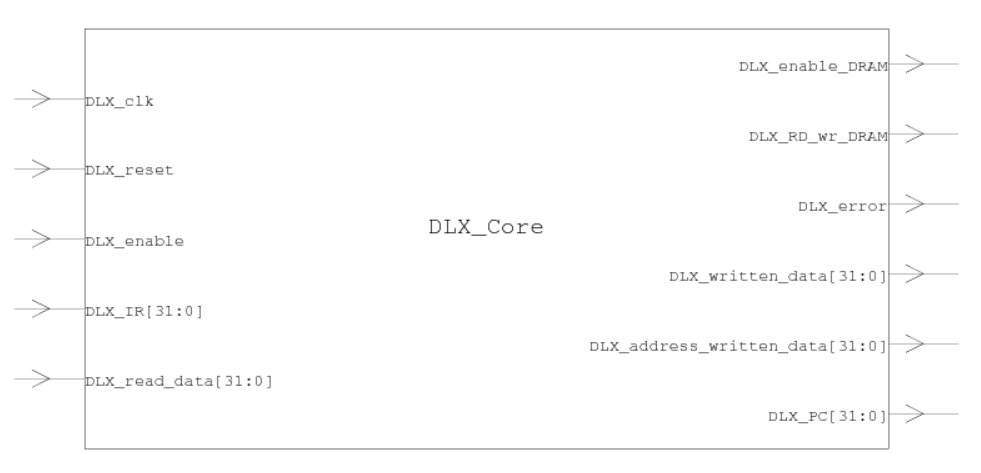
\includegraphics[scale=.6]{Immagini/05}
\label{02}
\caption{Core pinout}
\end{figure}

Just two informations about these signals. \textit{Clk} and \textit{enable} own their basic functionalities, \textit{IR} is the data read from the instruction RAM at each clock cycle by fetching. \textit{Read\_data} comes from the DRAM; \textit{enable\_DRAM} allows read and write operation on it, where the choice is made by \textit{RD\_wr\_RAM}. \textit{Error} is just a single pin out used for debugging, so not consider it. \textit{Written\_data} and \textit{address\_written\_data} are signals to the DRAM; in the end the \textit{PC} to the IRAM. \newline
The core is composed by 4 macroblocks:
\begin{itemize}
\item Datapath
\item Control unit
\item Branch target buffer
\item Branch misprediction manager
\end{itemize}
\begin{figure}[H]
\centering
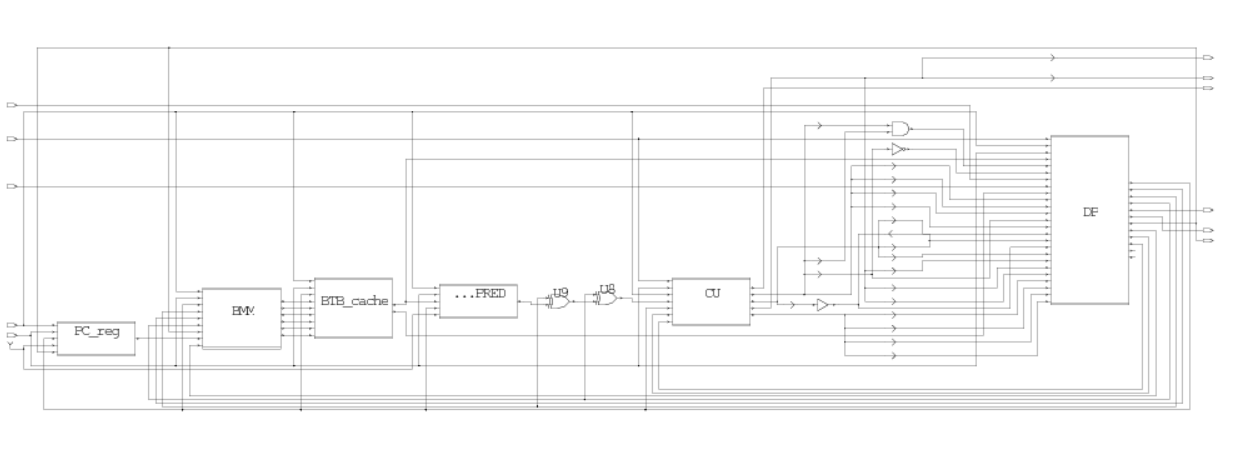
\includegraphics[scale=.6]{Immagini/06}
\label{02}
\caption{Core schematic - I}
\end{figure}

\begin{figure}[H]
\centering
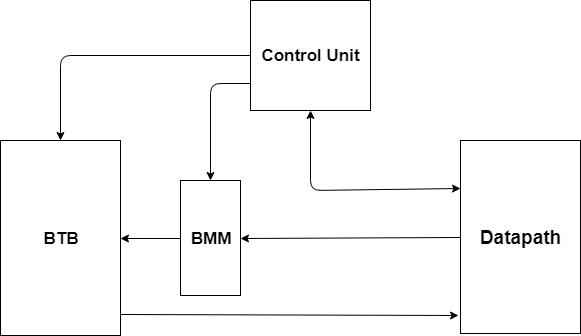
\includegraphics[scale=.6]{Immagini/07}
\label{02}
\caption{Core schematic - II}
\end{figure}
The datapath is the part of microprocessor computing instructions. In this design is the biggest component, where are defined the five pipeline stages. The branch target buffer is a sort of cache memory, used to manage control hazards; in fact branch addresses are stored in it. However almost all communications between datapath and BTB are managed by the Branch Misprediction Manager, which works when a wrong prediction occurs. Finally there is the hardwired Control Unit, that is the main brain of the DLX; as the datapath it's pipelined too.\newline
Datapath sends to BMM, so to BTB, information about the current instruction and the previous one such as: the program counter and whether one instruction is a branch or not. On the other side the BTB responds sending the branch target and the boolean value of the prediction (taken or untaken). The control unit oversees all macroblocks. It receives the instruction register of the instruction getting in the decode stage and produces all control signals.

\section{BTB}

I guess talking about BTB before datapath should let you understand better the overall behaviour of this microprocessor.